%================================================================
% SLO
%----------------------------------------------------------------
% datoteka: 	thesis_template.tex
%
% opis: 		predloga za pisanje diplomskega dela v formatu LaTeX na
% 				Univerza v Ljubljani, Fakulteti za računalništvo in informatiko
%
% pripravili: 	Matej Kristan, Zoran Bosnić, Andrej Čopar,
%			  	po začetni predlogi Gašperja Fijavža
%
% popravil: 	Domen Rački, Jaka Cikač, Matej Kristan
%
% verzija: 		30. september 2016 (dodan razširjeni povzetek)
%================================================================


%================================================================
% SLO: definiraj strukturo dokumenta
% ENG: define file structure
%================================================================
\documentclass[a4paper, 12pt]{book}

%================================================================
% SLO: Odkomentiraj "\SLOtrue " za izbiro slovenskega jezika
% ENG: Uncomment "\SLOfalse" to chose English languagge
%================================================================
\newif\ifSLO
% switch language

\SLOtrue % Enables Slovenian language
%\SLOfalse  % Enables English language

%================================================================
% SLO: vključi oblikovanje in pakete
% ENG: include design and packages
%================================================================
%----------------------------------------------------------------
% SLO: LaTeX paketi
% ENG: LateX packages
%----------------------------------------------------------------
% SLO: omogoča uporabo slovenskih (latinskih) črk kodiranih v formatu UTF-8
% ENG: enables the use of slovene (latin) caracters encoded in the UFT-8 format
\usepackage[utf8x]{inputenc}
%\inputencoding{utf8} 
% SLO: naloži, med drugim, slovenske delilne vzorce
% ENG: loads, among others, slovene dividing patterns
\usepackage[slovene,english]{babel} 
% SLO: poskrbi za postavitev strani
% ENG: takes care of the page layout
\usepackage{fancyhdr}
% SLO: za vlaganje slik različnih formatov
% ENG: for loading figures of different formats
\usepackage{graphicx}
\usepackage{caption}
\captionsetup[figure]{labelfont=bf} % SLO: napis "Slika #" v krepkem tisku
									% ENG: wirte "Figure #" caption in bold
\captionsetup[table]{labelfont=bf} % SLO: napis "Tabela #" v krepkem tisku
								   % ENG: wirte "Table #" caption in bold
% SLO: za pisanje psevdokode
% ENG: for writing pseudocode
\usepackage{algorithm}
\usepackage{algorithmic}
\floatname{algorithm}{\footnotesize Algorithm} % SLO: napis "Algoritem #" v krepkem tisku
											   % ENG: write "Algorithm #" caption in bold
% SLO: poveže reference slik/tabel in slike/tabele znotraj dokumenta
% ENG: links image/table references with the images/tables within the document
\usepackage[pdfa]{hyperref}
% SLO: pri kliku na referenco slike/tabele se postavi na vrh slike/tabele
% ENG: when clicking the image/table reference, position the focus on top of the image/table
\usepackage[all]{hypcap}
% SLO: omogoča, med drugim, definicjo in uporebo barve
% ENG: enables, among others, the definition and use of colors
\usepackage{xcolor}
%----------------------------------------------------------------
% SLO: dodatni paketi
% ENG: additional packages
%----------------------------------------------------------------
% SLO: omogoča večjo manipulacijo nad tabelami
% ENG: allows for greater manipulation of tables
\usepackage{booktabs}
% SLO: naloži dodatne simbole
% ENG: loads additional symbols
\usepackage{amssymb} 
% SLO: omogoča, med drugim, sklicevanje na formule z eqref
% ENG: enables, among others, equation referencing with eqref
\usepackage{amsmath}
% SLO: omogoča komentiranje večjega dela teksta
% ENG: enables the commenting of larger text parts
\usepackage{verbatim}
% SLO: omogoča rotacijo PDF strani v ležeč položaj
% ENG: enables the rotation of a PDF page to landscape
\usepackage{pdflscape}
% SLO: omogoča barvanje vrstic in stolpcev tabel
% ENG: enables coloring of table rows and columns
\usepackage{colortbl}
\usepackage{url}



%================================================================
% SLO: nastavitve dokumenta
% ENG: document properties
%================================================================
% SLO: prilagoditev robov za tisk
% ENG: margin adjustments for printing
\addtolength{\marginparwidth}{-20pt}
\addtolength{\oddsidemargin}{40pt}
\addtolength{\evensidemargin}{-40pt}
% SLO: razmik med vrsticami
% ENG: line spacing
\renewcommand{\baselinestretch}{1.3} 
% SLO: postavitev strani
% ENG: page layout
\renewcommand{\chaptermark}[1]{\markboth{\MakeUppercase{\thechapter.\ #1}}{}} 
\renewcommand{\sectionmark}[1]{\markright{\MakeUppercase{\thesection.\ #1}}} 
\renewcommand{\headrulewidth}{0.5pt} % Header rule
\renewcommand{\footrulewidth}{0pt} % Footer rule
%
\fancypagestyle{frontmatter}{%
	\fancyhf{} % Clear all headers and footers first
	\fancyhead[LE, RO]{\sl \thepage} 
	%\fancyhead[LO]{\sl \rightmark} 
	%\fancyhead[RE]{\sl \leftmark}
}
\fancypagestyle{mainmatter}{%
  	\fancyhf{} % Clear all headers and footers first
	\fancyhead[LE,RO]{\sl \thepage} 
	\fancyhead[LO]{\sl \rightmark} 
	\fancyhead[RE]{\sl \leftmark}
}
% SLO: font za ime avtorja
% ENG: font for author name
\newcommand{\authorfont}{\Large}
% SLO: font za naslov diplomskega dela
% ENG: font for thesis title
\newcommand{\titlefont}{\LARGE\bf}
% SLO: globina kazala
% ENG: content depth
\setcounter{tocdepth}{1}
% SLO: definiraj ukaz za prazno stran
% ENG: define the command for empty page
\newcommand{\clearemptydoublepage}{\newpage{\pagestyle{empty}\cleardoublepage}}

\newcommand{\BibTeX}{{\sc Bib}\TeX}


%----------------------------------------------------------------
% |||||||||||||||||||||| USTREZNO POPRAVI |||||||||||||||||||||||
% |||||||||||||||||||||| EDIT ACCORDINGLY |||||||||||||||||||||||
%----------------------------------------------------------------
\newcommand{\ttitle}{Vzorec zaključnega dela}
\newcommand{\ttitleEn}{Thesis template}
\newcommand{\tsubject}{\ttitle}
\newcommand{\tsubjectEn}{\ttitleEn}
\newcommand{\tauthor}{Mojster Jaka}
\newcommand{\temail}{mojster.jaka@gmai.com}
\newcommand{\myyear}{2016}
\newcommand{\tkeywords}{računalnik, računalnik, računalnik}
\newcommand{\tkeywordsEn}{computer, computer, computer}
\newcommand{\mysupervisor}{doc.~dr.\ Peter Klepec}
\newcommand{\mycosupervisor}{akad.~prof.~dr.\ Martin Krpan}

% include formatted front pages

%----------------------------------------------------------------
% SLO: definiraj metapodatke za datoteko thesis_template.tex
% ENG: define metadata for the file thesis_template.tex
%----------------------------------------------------------------
%----------------------------------------------------------------
%	HYPERREF SETUP
% SLO: ustrezno popravi e-mail
% ENG: edit the e-mail accordingly
%----------------------------------------------------------------
\hypersetup{pdftitle={\ttitle}}
\hypersetup{pdfsubject=\ttitleEn}
\hypersetup{pdfauthor={\tauthor, \temail}}
\hypersetup{pdfkeywords=\tkeywordsEn}

%----------------------------------------------------------------
% define medatata
% SLO: ustrezno popravi e-mail
% ENG: edit the e-mail accordingly
%----------------------------------------------------------------
\def\Title{\ttitle}
\def\Author{\tauthor, \temail}
\def\Subject{\ttitleEn}
\def\Keywords{\tkeywordsEn}
\def\Org{Univerza v Ljubljani, Fakulteta za računalništvo in informatiko}

%%%%%%%%%%%%%%%%%%%%%%%%%%%%%%%%%%%%%%%%
% \convertDate converts D:20080419103507+02'00' to 2008-04-19T10:35:07+02:00
%%%%%%%%%%%%%%%%%%%%%%%%%%%%%%%%%%%%%%%%
\def\convertDate{%
    \getYear
}

{\catcode`\D=12
 \gdef\getYear D:#1#2#3#4{\edef\xYear{#1#2#3#4}\getMonth}
}
\def\getMonth#1#2{\edef\xMonth{#1#2}\getDay}
\def\getDay#1#2{\edef\xDay{#1#2}\getHour}
\def\getHour#1#2{\edef\xHour{#1#2}\getMin}
\def\getMin#1#2{\edef\xMin{#1#2}\getSec}
\def\getSec#1#2{\edef\xSec{#1#2}\getTZh}
\def\getTZh +#1#2{\edef\xTZh{#1#2}\getTZm}
\def\getTZm '#1#2'{%
    \edef\xTZm{#1#2}%
    \edef\convDate{\xYear-\xMonth-\xDay T\xHour:\xMin:\xSec+\xTZh:\xTZm}%
}

\expandafter\convertDate\pdfcreationdate


%%%%%%%%%%%%%%%%%%%%%%%%%%%%%%%%%%%%%%%%
% get pdftex version string
%%%%%%%%%%%%%%%%%%%%%%%%%%%%%%%%%%%%%%%%
\newcount\countA
\countA=\pdftexversion
\advance \countA by -100
\def\pdftexVersionStr{pdfTeX-1.\the\countA.\pdftexrevision}

%%%%%%%%%%%%%%%%%%%%%%%%%%%%%%%%%%%%%%%%
% XMP data
%%%%%%%%%%%%%%%%%%%%%%%%%%%%%%%%%%%%%%%%
\usepackage{xmpincl}

%%%%%%%%%%%%%%%%%%%%%%%%%%%%%%%%%%%%%%%%
% pdfInfo
%%%%%%%%%%%%%%%%%%%%%%%%%%%%%%%%%%%%%%%%
\pdfinfo{%
    /Title    (\ttitle)
    /Author   (\tauthor, \temail)
    /Subject  (\ttitleEn)
    /Keywords (\tkeywordsEn)
    /ModDate  (\pdfcreationdate)
    /Trapped  /False
}

%================================================================
% SLO: razno
% ENG: other
%================================================================
% SLO: nastavitev sklicevanj
% ENG: hyper referencing setup
\definecolor{black}{rgb}{0,0,0}
\hypersetup{
	colorlinks = true,
	linkcolor = black,
	citecolor = black,
	urlcolor = black
}

%----------------------------------------------------------------
% SLO: dodaj poti do datotek s slikami, tabelami, ...
% ENG: add paths to files containing figures, tables, ...
%----------------------------------------------------------------
\graphicspath{
	{./figures/}
	{./tables/}
}
%----------------------------------------------------------------
% SLO: moji paketi
% ENG: my packages
%----------------------------------------------------------------
% ...
%----------------------------------------------------------------
% SLO: moji konstrukti
% ENG: my constructs
%----------------------------------------------------------------
\newtheorem{izrek}{Izrek}[chapter]
\newtheorem{trditev}{Trditev}[izrek]
\newenvironment{dokaz}{\emph{Dokaz.}\ }{\hspace{\fill}{$\Box$}}


%================================================================
% SLO: začetne strani magistrskega dela
% ENG: fist pages of the master's thesis
%================================================================
\begin{document}
% SLO: prepreči težave s številkami strani v kazalu
% ENG: prevents problems with the page numbers in the contents page
\renewcommand{\thepage}{}

%----------------------------------------------------------------
% Language-dependent formatting
%----------------------------------------------------------------
\ifSLO
    % SLO: definiraj slovensko besedo za kazalo
    \renewcommand{\contentsname}{Kazalo}

    % SLO: naslovnica  
    % select the course title if it exist
\ifTRACKEXIST
    \ifTRACKCS
        \renewcommand{\trackname}{Računalništvo in Informatika}
    \else
        \renewcommand{\trackname}{Podatkovne Vede}
    \fi
\fi

\ifPROGRAMMM
    \thispagestyle{empty}
    \begin{center}
        {\large\sc Univerza v Ljubljani\\Fakulteta za računalništvo in informatiko\\
            Fakulteta za elektrotehniko}
    	   \vskip 10em
    	   {\authorfont \tauthor \par}
    	   {\titlefont \ttitle \par}
        {\vskip 2em \textsc{MAGISTRSKO DELO\\[2mm]
        MAGISTRSKI PROGRAM DRUGE STOPNJE\\MULTIMEDIJA
        }\par}
        \vfill\null
        {\large \textsc{Mentor}: \mysupervisor \par}
   	    {\large \textsc{Somentor}: \mycosupervisor \par}
        {\vskip 2em \large Ljubljana, \myyear \par}
   \end{center}
\else
    \thispagestyle{empty}
	\begin{center}
            {\large\sc Univerza v Ljubljani\\Fakulteta za računalništvo in informatiko}
    	   \vskip 10em
    	   {\authorfont \tauthor \par}
    	   {\titlefont \ttitle \par}
        {\vskip 2em \textsc{MAGISTRSKO DELO\\[2mm]
        MAGISTRSKI PROGRAM DRUGE STOPNJE\\RAČUNALNIŠTVO IN INFORMATIKA
        \ifTRACKEXIST
            \\Smer: \trackname
        \fi
        }\par}
        \vfill\null
        {\large \textsc{Mentor}: \mysupervisor \par}
   	    {\large \textsc{Somentor}: \mycosupervisor \par}
        {\vskip 2em \large Ljubljana, \myyear \par}
   \end{center}
\fi  \clearemptydoublepage
    % SLO: avtorske pravice
    \thispagestyle{empty}
\vspace*{\fill}
{\noindent\footnotesize
{\sc Avtorske pravice}. 
\ifPROGRAMMM
    Rezultati magistrskega dela so intelektualna lastnina avtorja, Fakultete za ra\-ču\-nal\-niš\-tvo in informatiko ter Fakultete za Elektrotehniko Univerze v Ljubljani. Za objavljanje ali izkoriščanje rezultatov ma\-gi\-str\-ske\-ga dela je potrebno pisno soglasje avtorja, Fakultete za ra\-ču\-nal\-niš\-tvo in informatiko, Fakultete za Elektrotehniko ter mentorja\footnote{V dogovorju z mentorjem lahko kandidat magistrsko delo s pripadajočo izvorno kodo izda tudi pod drugo licenco, ki ponuja določen del pravic vsem: npr. Creative Commons, GNU GPL. V tem primeru na to mesto vstavite opis licence, na primer tekst~\cite{licence}.}.
\else
    Rezultati magistrskega dela so intelektualna lastnina avtorja in Fakultete za ra\-ču\-nal\-niš\-tvo in informatiko Univerze v Ljubljani. Za objavljanje ali izkoriščanje rezultatov ma\-gi\-str\-ske\-ga dela je potrebno pisno soglasje avtorja, Fakultete za ra\-ču\-nal\-niš\-tvo in informatiko ter mentorja\footnote{V dogovorju z mentorjem lahko kandidat magistrsko delo s pripadajočo izvorno kodo izda tudi pod drugo licenco, ki ponuja določen del pravic vsem: npr. Creative Commons, GNU GPL. V tem primeru na to mesto vstavite opis licence, na primer tekst~\cite{licence}.}.
\fi    
}
\begin{center}
{\footnotesize{\sc \copyright \myyear\ \tauthor}}
\end{center}  \clearemptydoublepage
    % SLO: izjava o avtorstvu (ni več del vezane izdaje, ločena oddaja)
    % SLO: zahvala
    \thispagestyle{empty}

\begin{center}
{\Large \textbf{\sc Zahvala}}
\end{center}
\vspace{0.5cm}

{\it\noindent
Na tem mestu zapišite, komu se zahvaljujete za izdelavo magistrske naloge. V zahvali se poleg mentorja spodobi omeniti vse, ki so s svojo pomočjo prispevali k nastanku vašega izdelka.

\vspace{0.5cm} \hfill \tauthor, \myyear
} \clearemptydoublepage
    % SLO: posvetilo
    \thispagestyle{empty}\mbox{}{\vskip0.20\textheight}\mbox{}\hfill\begin{minipage}{0.55\textwidth}%

Vsem rožicam tega sveta.\\\\
\textit{''The only reason for time is so that everything doesn't happen at once.''}
\flushright --- Albert Einstein
\normalfont\end{minipage} \clearemptydoublepage
\else
    % ENG: title page ENG
    % select the course title if it exist
\ifTRACKEXIST
    \ifTRACKCS
        \renewcommand{\trackname}{Computer and Information Science}
    \else
        \renewcommand{\trackname}{Data Science}
    \fi
\fi

\ifPROGRAMMM
    \thispagestyle{empty}
	\begin{center}
        {\large\sc University of Ljubljana\\Faculty of Computer and Information Science\\
        Faculty of Electrical Engineering}
    	\vskip 10em
    	{\authorfont \tauthor \par}
    	{\titlefont \ttitleEn \par}
        {\vskip 2em \textsc{MASTER'S THESIS\\[2mm]
        THE 2nd CYCLE MASTER'S STUDY PROGRAMME\\MULTIMEDIA
        }\par}
        \vfill\null
        {\large \textsc{Supervisor}: \mysupervisor \par}
   	    {\large \textsc{Co-supervisor}:  \mycosupervisor \par}
        {\vskip 2em \large Ljubljana, \myyear \par}
   \end{center}
\else
    \thispagestyle{empty}
	\begin{center}
        {\large\sc University of Ljubljana\\Faculty of Computer and Information Science}
    	\vskip 10em
    	{\authorfont \tauthor \par}
    	{\titlefont \ttitleEn \par}
        {\vskip 2em \textsc{MASTER'S THESIS\\[2mm]
        THE 2nd CYCLE MASTER'S STUDY PROGRAMME\\COMPUTER AND INFORMATION SCIENCE
        \ifTRACKEXIST
            \\Track: \trackname
        \fi
        }\par}
        \vfill\null
        {\large \textsc{Supervisor}: \mysupervisor \par}
   	    {\large \textsc{Co-supervisor}:  \mycosupervisor \par}
        {\vskip 2em \large Ljubljana, \myyear \par}
    \end{center}
\fi  \clearemptydoublepage
    % ENG: title page SLO
    % select the course title if it exist
\ifTRACKEXIST
    \ifTRACKCS
        \renewcommand{\trackname}{Računalništvo in Informatika}
    \else
        \renewcommand{\trackname}{Podatkovne Vede}
    \fi
\fi

\ifPROGRAMMM
    \thispagestyle{empty}
    \begin{center}
        {\large\sc Univerza v Ljubljani\\Fakulteta za računalništvo in informatiko\\
            Fakulteta za elektrotehniko}
    	   \vskip 10em
    	   {\authorfont \tauthor \par}
    	   {\titlefont \ttitle \par}
        {\vskip 2em \textsc{MAGISTRSKO DELO\\[2mm]
        MAGISTRSKI PROGRAM DRUGE STOPNJE\\MULTIMEDIJA
        }\par}
        \vfill\null
        {\large \textsc{Mentor}: \mysupervisor \par}
   	    {\large \textsc{Somentor}: \mycosupervisor \par}
        {\vskip 2em \large Ljubljana, \myyear \par}
   \end{center}
\else
    \thispagestyle{empty}
	\begin{center}
            {\large\sc Univerza v Ljubljani\\Fakulteta za računalništvo in informatiko}
    	   \vskip 10em
    	   {\authorfont \tauthor \par}
    	   {\titlefont \ttitle \par}
        {\vskip 2em \textsc{MAGISTRSKO DELO\\[2mm]
        MAGISTRSKI PROGRAM DRUGE STOPNJE\\RAČUNALNIŠTVO IN INFORMATIKA
        \ifTRACKEXIST
            \\Smer: \trackname
        \fi
        }\par}
        \vfill\null
        {\large \textsc{Mentor}: \mysupervisor \par}
   	    {\large \textsc{Somentor}: \mycosupervisor \par}
        {\vskip 2em \large Ljubljana, \myyear \par}
   \end{center}
\fi  \clearemptydoublepage
    % ENG: copyright
    \thispagestyle{empty}
\vspace*{\fill}
{\noindent\footnotesize
{\sc Copyright}. 
\ifPROGRAMMM
    The results of this master's thesis are the intellectual property of the author, the Faculty of Computer and Information Science and the Faculty of Electrical Engineering, University of Ljubljana. For the publication or exploitation of the master's thesis results, a written consent of the author, the Faculty of Computer and Information Science, the Faculty of Electrical Engineering and the supervisor is necessary.
    \footnote{V dogovorju z mentorjem lahko kandidat magistrsko delo s pripadajočo izvorno kodo izda tudi pod drugo licenco, ki ponuja določen del pravic vsem: npr. Creative Commons, GNU GPL. V tem primeru na to mesto vstavite opis licence, na primer tekst~\cite{licence}.}
\else
    The results of this master's thesis are the intellectual property of the author and the Faculty of Computer and Information Science, University of Ljubljana. For the publication or exploitation of the master's thesis results, a written consent of the author, the Faculty of Computer and Information Science, and the supervisor is necessary.
    \footnote{V dogovorju z mentorjem lahko kandidat magistrsko delo s pripadajočo izvorno kodo izda tudi pod drugo licenco, ki ponuja določen del pravic vsem: npr. Creative Commons, GNU GPL. V tem primeru na to mesto vstavite opis licence, na primer tekst~\cite{licence}.}
\fi    
}
\begin{center}
{\footnotesize{\sc \copyright \myyear\ \tauthor}}
\end{center}  \clearemptydoublepage
    % ENG: declaration of authorship (not part of paper edition, turn in separately)
    % ENG: acknowledgements
    \thispagestyle{empty}

\begin{center}
{\Large \textbf{\sc Acknowledgments}}
\end{center}
\vspace{0.5cm}

{\it\noindent
Worth mentioning in the acknowledgment is everyone who contributed to your thesis.

\vspace{0.5cm} \hfill \tauthor, \myyear
} \clearemptydoublepage
    % ENG: dedication
    \thispagestyle{empty}\mbox{}{\vskip0.20\textheight}\mbox{}\hfill\begin{minipage}{0.55\textwidth}%

To all the flowers of this world.\\\\
\textit{''The only reason for time is so that everything doesn't happen at once.''}
\flushright --- Albert Einstein
\normalfont\end{minipage} \clearemptydoublepage
\fi

%----------------------------------------------------------------
% SLO: kazalo
% ENG: contents
%----------------------------------------------------------------
\begingroup
	\hypersetup{colorlinks=true,linkcolor=black}
	\def\thepage{}
	\tableofcontents{}
	\clearemptydoublepage
\endgroup


\ifSLO
    % SLO: seznam kratic
    \chapter*{Seznam uporabljenih kratic}

\begin{tabular}{l|l|l}
  {\bf kratica} & {\bf angleško} & {\bf slovensko} \\ \hline
  % after \\: \hline or \cline{col1-col2} \cline{col3-col4} ...
  {\bf CA} & classification accuracy & klasifikacijska točnost \\
  {\bf DBMS} & database management system & sistem za upravljanje podatkovnih baz \\
  {\bf SVM} & support vector machine & metoda podpornih vektorjev \\
  ... & ... & ... \\
\end{tabular} \clearemptydoublepage
    % SLO: glavne strani diplomskega dela
\else
    % ENG: list of acronmys
    \chapter*{List of used acronmys}

\begin{tabular}{l|l|l}
  {\bf acronym} & {\bf meaning}  \\ \hline
  % after \\: \hline or \cline{col1-col2} \cline{col3-col4} ...
  {\bf CA} & classification accuracy \\
  {\bf DBMS} & database management system \\
  {\bf SVM} & support vector machine \\
  ... & ... \\
\end{tabular} \clearemptydoublepage
\fi

\frontmatter
\pagestyle{frontmatter}
\setcounter{page}{1} %
\renewcommand{\thepage}{}       % preprecimo težave s številkami strani v kazalu
 
% Include extended abstract [Razširjeni povzetek v slovenščini-- le za dela pisana v angleščini]
\ifSLO
    % include Slovenian abstract
    %---------------------------------------------------------------
% SLO: slovenski povzetek
% ENG: slovenian abstract
%---------------------------------------------------------------
\selectlanguage{slovene} % Preklopi na slovenski jezik
\addcontentsline{toc}{chapter}{Povzetek}
\chapter*{Povzetek}

\noindent\textbf{Naslov:} \ttitle
\bigskip

V vzorcu je predstavljen postopek priprave magistrskega dela z uporabo okolja \LaTeX. Vaš povzetek mora sicer vsebovati približno 100 besed, ta tukaj je odločno prekratek. Dober povzetek vključuje: (1) kratek opis obravnavanega problema, (2) kratek opis vašega pristopa za reševanje tega problema in (3) (najbolj uspešen) rezultat ali prispevek magistrske naloge.

\subsection*{Ključne besede}
\textit{\tkeywords}
\clearemptydoublepage
    % include English abstract
     %---------------------------------------------------------------
% SLO: angleški povzetek
% ENG: english abstract
%---------------------------------------------------------------
\selectlanguage{english} % Preklopi na angleški jezik
\addcontentsline{toc}{chapter}{Abstract}
\chapter*{Abstract}

\noindent\textbf{Title:} \ttitleEn
\bigskip

This sample document presents an approach to typesetting your BSc thesis using \LaTeX. A proper abstract should contain around 100 words which makes this one way too short. A good abstract contains: (1) a short description of the tackled problem, (2) a short description of your approach to solving the problem, and (3) (the most successful) result or contribution in your thesis.

\subsection*{Keywords}
\textit{\tkeywordsEn}
\clearemptydoublepage
\else
    % include English abstract
     %---------------------------------------------------------------
% SLO: angleški povzetek
% ENG: english abstract
%---------------------------------------------------------------
\selectlanguage{english} % Preklopi na angleški jezik
\addcontentsline{toc}{chapter}{Abstract}
\chapter*{Abstract}

\noindent\textbf{Title:} \ttitleEn
\bigskip

This sample document presents an approach to typesetting your BSc thesis using \LaTeX. A proper abstract should contain around 100 words which makes this one way too short. A good abstract contains: (1) a short description of the tackled problem, (2) a short description of your approach to solving the problem, and (3) (the most successful) result or contribution in your thesis.

\subsection*{Keywords}
\textit{\tkeywordsEn}
\clearemptydoublepage
    % include Slovenian abstract
    %---------------------------------------------------------------
% SLO: slovenski povzetek
% ENG: slovenian abstract
%---------------------------------------------------------------
\selectlanguage{slovene} % Preklopi na slovenski jezik
\addcontentsline{toc}{chapter}{Povzetek}
\chapter*{Povzetek}

\noindent\textbf{Naslov:} \ttitle
\bigskip

V vzorcu je predstavljen postopek priprave magistrskega dela z uporabo okolja \LaTeX. Vaš povzetek mora sicer vsebovati približno 100 besed, ta tukaj je odločno prekratek. Dober povzetek vključuje: (1) kratek opis obravnavanega problema, (2) kratek opis vašega pristopa za reševanje tega problema in (3) (najbolj uspešen) rezultat ali prispevek magistrske naloge.

\subsection*{Ključne besede}
\textit{\tkeywords}
\clearemptydoublepage
  
  %  \cleardoublepage
    \let\oldthesection=\thesection %Special section numbering for this chapter - remember default one
    \let\oldthesubsection=\thesubsection
    \renewcommand{\thesection}{\Roman{section}} %Special section numbering for this chapter
    \renewcommand{\thesubsection}{\thesection.\Roman{subsection}}

    % set roman page numbering
    \pagenumbering{roman}
    % set slovene language
    \selectlanguage{slovene}
    % insert extended abstract
     \chapter{Razširjeni povzetek}
 
 To je primer razširjenega povzetka v slovenščini, ki je obvezen za naloge pisane v angleščini. Razširjeni povzetek mora vsebovati vse glavne elemente dela napisanega v angleščini skupaj s kratkim uvodom in povzetkom glavnih elementov metode, glavnih eksperimentalnih rezultatov in glavnih ugotovitev. Razširjeni povzetek naj bo strukturiran v podpoglavja (spodaj je naveden le okvirni primer in je nezavezujoč).
 Čez palec navadno razširjeni povzetek nanese okoli 10 odstotkov obsega celotnega dela. 
 
 \section{Kratek pregled sorodnih del}
 
 \section{Predlagana metoda}
 
 \section{Eksperimentalna evaluacija}
 
 \section{Sklep}
 
poljuben tekst  poljuben tekst  poljuben tekst  poljuben tekst  poljuben tekst  poljuben tekst  poljuben tekst  poljuben tekst  poljuben tekst  poljuben tekst  poljuben tekst  poljuben tekst  poljuben tekst  poljuben tekst  poljuben tekst  poljuben tekst  poljuben tekst  poljuben tekst  poljuben tekst  poljuben tekst  poljuben tekst  poljuben tekst  poljuben tekst  poljuben tekst  poljuben tekst  poljuben tekst  poljuben tekst  poljuben tekst  poljuben tekst  poljuben tekst  poljuben tekst  poljuben tekst  poljuben tekst  poljuben tekst  poljuben tekst  poljuben tekst  poljuben tekst  poljuben tekst  poljuben tekst  poljuben tekst  poljuben tekst  poljuben tekst  poljuben tekst  poljuben tekst  poljuben tekst  poljuben tekst  poljuben tekst  poljuben tekst  poljuben tekst  poljuben tekst  poljuben tekst  poljuben tekst  poljuben tekst  poljuben tekst  poljuben tekst  poljuben tekst  poljuben tekst  poljuben tekst  poljuben tekst  poljuben tekst  poljuben tekst  poljuben tekst  poljuben tekst  poljuben tekst  poljuben tekst  poljuben tekst  poljuben tekst  poljuben tekst  poljuben tekst  poljuben tekst  poljuben tekst  poljuben tekst  poljuben tekst  poljuben tekst  poljuben tekst  poljuben tekst  poljuben tekst  poljuben tekst  poljuben tekst  poljuben tekst  poljuben tekst  poljuben tekst  poljuben tekst  poljuben tekst  poljuben tekst  poljuben tekst  poljuben tekst  poljuben tekst  poljuben tekst  poljuben tekst 


    \let\thesection=\oldthesection % Restore default section numbering
    \let\thesubsection=\oldthesubsection
\fi

%----------------------------------------------------------------
% SLO: Preklopi izbrani jezik
% ENG: Switch to chosen language
%----------------------------------------------------------------
\ifSLO
    \selectlanguage{slovene} % Preklopi na slovenski jezik
\else
    \selectlanguage{english}  % Switch to english language
\fi

% SLO: vklopi številčenje poglavji, ponastavi številčenje strani in uporabi arabske številkami za številčenje strani
% ENG: turns on chapter numbering, resets page numbering and uses arabic numerals for page numbers
\mainmatter
\pagestyle{mainmatter}
\setcounter{page}{1}
\pagestyle{fancy}


%================================================================
% ENG: main pages of the thesis
%================================================================

%----------------------------------------------------------------
% Poglavje (Chapter) 1
%----------------------------------------------------------------
\chapter{Uvod}
\label{ch:uvod}

Datoteka {\tt magistrska\_naloga.tex} na kratko opisuje, kako se pisanja magistrskega dela lotimo z uporabo programskega pateka \LaTeX. V tem dokumentu bomo predstavili nekaj njegovih prednosti in hib. Kar se slednjih tiče, mi pride na misel ena sama. Ko se srečamo z njim, nam izgleda kot kislo jabolko, nismo prepričani, da bi želeli vanj ugrizniti. Lahko pa z njim pripravimo odličen zavitek ali pa pridemo na okus.

V Poglavju~\ref{ch:uvod} bomo na hitro spoznali besedilne konstrukte kot so izreki, enačbe in dokazi. Naučili se bomo, kako se na njih sklicujemo. V Poglavju~\ref{ch:sklicevanje} se bomo srečali s sklicevanjem na besedilne konstrukte. Poglavje~\ref{ch:plovke} bo predstavilo vključevanje plovk: slik in tabel. V Poglavju~\ref{ch3} se bomo srečali s sklicevanjem na literaturo.
Sledil bo samo še zaključek.

Bodite pozorni, da se v glavni mapi nahajata še datoteki \verb+ declaration.tex+ in \verb+ izjava.tex+. Ti datoteki se ločeno prevedeta, ju podpišete in oddate v referat ločeno od magistrske naloge.

%----------------------------------------------------------------
% Poglavje (Chapter) 2
%----------------------------------------------------------------
\chapter{Sklicevanje na besedilne konstrukte}
\label{ch:sklicevanje}

Matematična ali popolna indukcija je eno prvih orodij, ki jih spoznamo za dokazovanje trditev pri matematičnih predmetih.
\begin{izrek}
\label{iz:1}
Za vsako naravno število $n$ velja
\begin{equation}
n < 2^n.
\label{eq:1}
\end{equation}
\end{izrek}
\begin{dokaz}
Dokazovanje z indukcijo zahteva, da neenakost~\eqref{eq:1} najprej preverimo za najmanjše naravno število --- $0$. Res, ker je $0 < 1 = 2^0$, je neenačba~\eqref{eq:1} za $n=0$ izpolnjena.

Sledi indukcijski korak. S predpostavko, da je neenakost~\eqref{eq:1} veljavna pri nekem naravnem številu $n$, je potrebno pokazati, da je ista neenakost v veljavi tudi pri njegovem nasledniku --- naravnem številu $n+1$. Izračun zapišemo s tremi vrsticami, ki jih končamo s piko, saj do del tega stavka:
\begin{align}
n+1 &< 2^n + 1,  \label{eq:2}\\
    &\le 2^n + 2^n, \label{eq:3}\\
    &= 2^{n+1}. \nonumber
\end{align}
Neenakost~\eqref{eq:2} je posledica indukcijske predpostavke, neenakost~\eqref{eq:3} pa enostavno dejstvo, da je za vsako naravno število $n$ izraz $2^n$ vsaj tako velik kot 1. S tem je dokaz Izreka~\ref{iz:1} zaključen.
\end{dokaz}

Opazimo, da je \LaTeX\ številko izreka podredil številki poglavja.



%----------------------------------------------------------------
% Poglavje (Chapter) 3
%----------------------------------------------------------------
\chapter{Plovke: slike in tabele}
\label{ch:plovke}

Slike in daljše tabele praviloma vključujemo v dokument kot plovke. Pozicija plovke v končnem izdelku ni pogojena s tekom besedila, temveč z izgledom strani. \LaTeX\ bo skušal plovko postaviti samostojno, praviloma na vrh strani, na kateri se na takšno plovko prvič sklicujemo. Pri tem pa bo na vsako stran končnega izdelka želel postaviti tudi sorazmerno velik del besedila. V skrajnem primeru, če imamo res preveč plovk, se bo odločil za stran popolnoma zapolnjeno s plovkami.

\section{Formati slik}
Bitne slike, vektorske slike, kakršnekoli slike, z \LaTeX{}om lahko vključimo vse.
Slika~\ref{pic1} je v {\tt .pdf} formatu.
\begin{figure}
    \begin{center}
        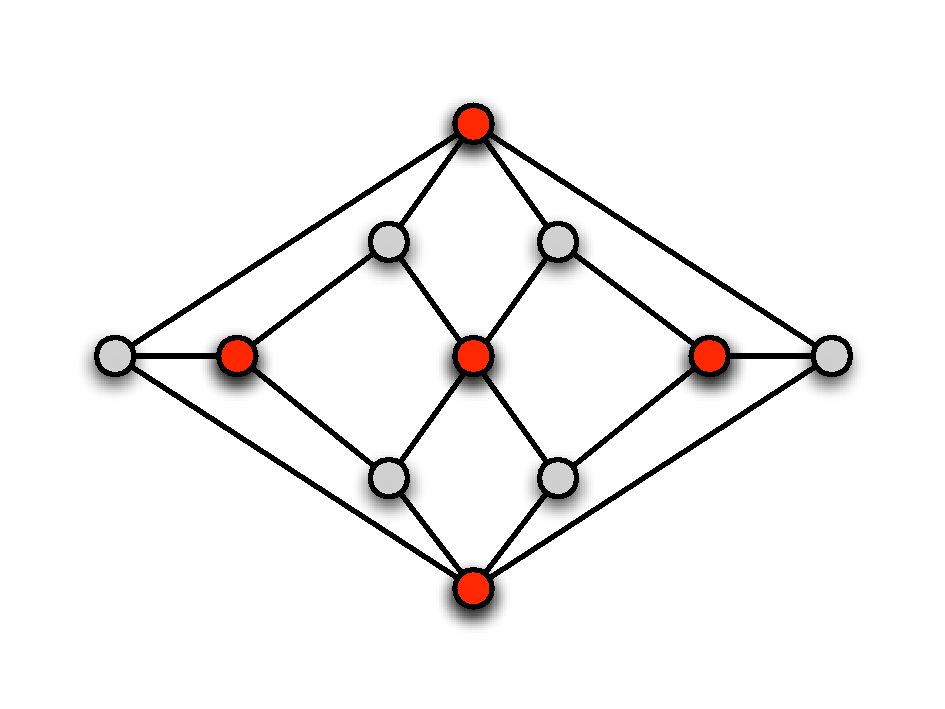
\includegraphics[width=10cm]{pic1.pdf}
    \end{center}
\caption{Herschelov graf, vektorska grafika.}
\label{pic1}
\end{figure}
Pa res lahko vključimo slike katerihkoli formatov? Žal ne. Programski paket \LaTeX\ lahko uporabljamo v več dialektih. Ukaz {\tt latex} ne mara vključenih slik v formatu Portable Document Format {\tt .pdf}, ukaz {\tt pdflatex} pa ne prebavi slik v Encapsulated Postscript Formatu {\tt .eps}.
Strnjeno v Tabeli~\ref{tbl:1}.

\begin{table}
\caption{}
    \begin{center}
        \begin{tabular}{l|ccc}
            ukaz/format & {\tt .pdf} & {\tt .eps} & ostali formati \\ \hline
                        {\tt pdflatex} & da & ne & da \\
                        {\tt latex}   & ne & da  & da
        \end{tabular}
    \end{center}
\label{tbl:1}
\end{table}

Nasvet? Odločite se za uporabo ukaza {\tt pdflatex}. Vaš izdelek bo brez vmesnih stopenj na voljo v {.pdf} formatu in ga lahko odnesete v vsako tiskarno. Če morate na vsak način vključiti sliko, ki jo imate v {\tt .eps} formatu, jo vnaprej pretvorite v alternativni format, denimo {\tt .pdf}.

Včasih se da v okolju za uporabo programskega paketa \LaTeX\ nastaviti na kakšen način bomo prebavljali vhodne dokumente. Spustni meni na Sliki~\ref{pic2} odkriva uporabo \LaTeX{}a v njegovi pdf inkarnaciji --- {\tt pdflatex}.
\begin{figure}
\begin{center}
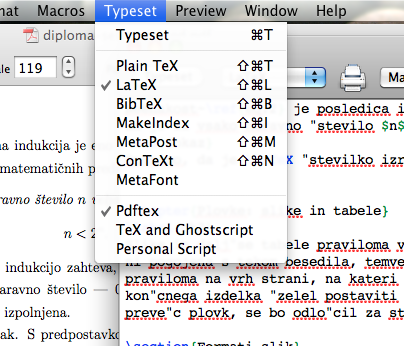
\includegraphics[width=10cm]{pic2.png}
\end{center}
\caption{Kateri dialekt uporabljati?}
\label{pic2}
\end{figure}
Vključena Slika~\ref{pic2} je seveda bitna.



%----------------------------------------------------------------
% Poglavje (Chapter) 4
%----------------------------------------------------------------
\chapter{Razno}
\label{ch:razno}

\section{Notacije}
\label{sec:notacije}

Za notacijo spremenljivk ter skalarjev uporabimo običajno notacijo, t.j., spremenljivka $x$ in skalar $a$. Pri notaciji matrik ter vektorjev pa se poslužujemo krepega fonta. Torej, matrika $\boldsymbol{A}$ ter vektor $\boldsymbol{v}$,
\begin{equation}
\boldsymbol{A} = \begin{bmatrix}
       a_{11} & a_{12} & \dots & a_{1q}  \\
       a_{21} & a_{22} & \dots & a_{2q}  \\
       \vdots  \\
       a_{p1} & a_{p2} & \dots & a_{pq}  \\
     \end{bmatrix}, \quad
     \boldsymbol{v} = \begin{bmatrix}
       x_1  \\
       x_2  \\
       \vdots  \\
       x_q  \\
     \end{bmatrix}. \nonumber
\end{equation}

%----------------------------------------------------------------
\section{Lepe tabele in psevdokoda}
\label{sec:psevdokoda}

Psevdokoda~\ref{alg:primer} prikazuje primer delovanja genetskega algoritma, medtem ko Tabela~\ref{tab:params} prikazuje primer lepe tabele brez vertikalnih črt.

\begin{algorithm}
\caption{Psevdokoda genetskega algoritma}
\label{alg:primer}
\begin{algorithmic}[1]
\footnotesize
\STATE $t \gets 0$
\STATE $InitPopulation[P(t)] \gets$ inicializiraj populacijo
\STATE $EvalPopulation[P(t)] \gets$ evaluiraj populacijo
\REPEAT
\STATE $P'(t) \gets Variation[P(t)] \gets $ generiraj novo populacijo
\STATE $EvalPopulation[P'(t)] \gets$ evaluiraj novo populacijo
\STATE $P(t+1) \gets ApplyGeneticOperators[P'(t) \in Q]$
\STATE $t \gets t+1$
\UNTIL{prekinitev}
\IF{rezultat dovolj dober}
\STATE shrani rezultat
\ENDIF
\end{algorithmic}
\end{algorithm}

%---------------------------------------------------------------
\begin{table}
\caption{Primer enostavne tabele.}
\centering
\scalebox{0.82}{
\begin{tabular}{c c c}
 \toprule
 Ime & Vrednost & Opis \\
 \midrule
 \textit{ $a$ } & 0.03 &  skalar \\
 \textit{ $x$ } & -1 & spremenljivka \\
 \bottomrule
\end{tabular}
}
\label{tab:params}
\end{table}

%----------------------------------------------------------------
% Poglavje (Chapter) 5
%----------------------------------------------------------------
\chapter{Kaj pa literatura?}
\label{ch3}
Kot smo omenili že v uvodu, je pravi način za citiranje literature uporaba \BibTeX{}a~\cite{ubi}.
Programski paket \LaTeX je prvotno predstavljen v priročniku~\cite{Lamport} in je v resnici nadgradnja sistema \TeX\ avtorja Donalda Knutha, znanega po denimo, če izpustim njegovo umetnost programiranja, Knuth-Bendixovem algoritmu~\cite{Knuth}.

Vsem raziskovalcem s področja računalništva pa svetujem v branje mnenje L.\ Fortnowa~\cite{Fortnow}.

%----------------------------------------------------------------
% Poglavje (Chapter) 6
%----------------------------------------------------------------
\chapter{Sklepne ugotovitve}
Izbira \LaTeX\ ali ne \LaTeX\ je seveda prepuščena vam samim. Res je, da so prvi koraki v \LaTeX{}u težavni. Ta dokument naj vam služi kot začetna opora pri hoji.

% ---------------------------------------------------------------
% Appendix
% ---------------------------------------------------------------
\appendix
%\addcontentsline{toc}{chapter}{Razširjeni povzetek}
\chapter{Title of the appendix 1}

Example of the appendix.

%----------------------------------------------------------------
% SLO: bibliografija
% ENG: bibliography
%----------------------------------------------------------------
\bibliographystyle{elsarticle-num}

%----------------------------------------------------------------
% SLO: odkomentiraj za uporabo zunanje datoteke .bib (ne pozabi je potem prevesti!)
% ENG: uncomment to use .bib file (don't forget to compile it!)
%----------------------------------------------------------------
%\bibliography{bibliography}

%----------------------------------------------------------------
% SLO: zakomentiraj spodnji del, če uporabljaš zunanjo .bib datoteko
% ENG: comment the part below if using the .bib file
%----------------------------------------------------------------

\begin{thebibliography}{99}
\bibitem{Fortnow} L.\ Fortnow, ``Viewpoint: Time for computer science to grow up'',
{\it Communications of the ACM}, št.\ 52, zv.\ 8, str.\ 33--35, 2009.
\bibitem{Knuth} D.\ E.\ Knuth, P. Bendix. ``Simple word problems in universal algebras'', v zborniku: Computational Problems in Abstract Algebra (ur. J. Leech), 1970, str. 263--297.
\bibitem{Lamport} L.\ Lamport. {\it LaTEX: A Document Preparation System}. Addison-Wesley, 1986.
\bibitem{ubi} O.\ Patashnik (1998) \BibTeX{}ing.
Dostopno na: \url{http://ftp.univie.ac.at/packages/tex/biblio/bibtex/contrib/doc/btxdoc.pdf}
\bibitem{licence} licence-cc.pdf. Dostopno na: \url{https://ucilnica.fri.uni-lj.si/course/view.php?id=274}
\end{thebibliography}

\end{document}
